
\documentclass[10pt]{article}

\usepackage{graphicx,amsmath,amssymb,subfigure,enumerate,versions}
\usepackage{multicol,multirow,mdframed}
\usepackage{epstopdf}
\usepackage{pstricks,auto-pst-pdf}
\usepackage{pst-all}
\usepackage{pst-ode}
\usepackage{pst-math}
\usepackage{hyperref}
\usepackage{listings}
%\usepackage{mcode}
\lstset{language=Matlab}
\DeclareGraphicsExtensions{.png,.jpg,.pdf}

% ************ Page Margins *************
\hoffset=-1.3in
\setlength{\textwidth}{7.5in}
%%%%% MARGINS
\topmargin 0pt
\advance \topmargin by -\headheight
\advance \topmargin by -\headsep
\textheight 9.5in

% ************ Shortcuts *************
\newcommand{\Z}{\mbox{\sf Z\hspace{-1.5mm}Z}}
\newcommand{\SolutionSeparator}{ \hfill \hfill \hrule \hfill \hfill }
\newcommand{\R}{\mbox{\rm I\hspace{-0.75mm}R}}
\columnsep=0.75in
\newcommand{\vsc}{\vspace{1mm}}
\newcommand{\D}{\Delta }
\newcommand{\ifd}{f(x)~dx}
\newcommand{\dd}{\frac{dy}{dx} \,} 
\newcommand{\der}[2]{\frac{d{#1}}{d{#2}} \,}
\newcommand{\ddx}[1]{\frac{d {#1}}{dx} \,} 
\newcommand{\ddy}[1]{\frac{d {#1}}{dy} \,} 
\newcommand{\ddz}[1]{\frac{d {#1}}{dz} \,} 
\newcommand{\ddt}[1]{\frac{d {#1}}{dt} \,} 
\newcommand{\ds}{\displaystyle } 
\newcommand{\la}{\lambda } 
\newcommand{\del}{\nabla } 
\newcommand{\zx}{\frac{\partial z}{\partial x} \,}
\newcommand{\zy}{\frac{\partial z}{\partial y} \,}
\newcommand{\dx}{\frac{\partial f}{\partial x} \,}
\newcommand{\dy}{\frac{\partial f}{\partial y} \,}
\newcommand{\pp}[2]{\frac{\partial {#1}}{\partial {#2}} \,}
\newcommand{\ppx}{\frac{\partial }{\partial x} \,}
\newcommand{\ppy}{\frac{\partial }{\partial y} \,}
\renewcommand{\thesection}{\Roman{section}}
\newcommand{\vi}{\vec{i}}
\newcommand{\vj}{\vec{j}}
\newcommand{\vk}{\vec{k}}
\newcommand{\vv}{\vec{v}}
\newcommand{\lan}{\left\langle}
\newcommand{\ran}{\right\rangle}
\newcommand{\degr}{^{\circ}}

% *** Define the printed question style ***
\newcommand{\q}[1]{ {\em #1} }
% \renewcommand{\q}[1]{ {} }

\newcommand{\notice}{ \begin{center}Some problems and solutions
    selected or adapted from \\ Stewart {\em Calculus-Early
      Transcendentals} and Hughes-Hallett {\em Calculus} .\end{center}
}

% *** Overwrite, if desired, the question format
\includeversion{Question} 
\includeversion{Solution}

\newcommand{\multicolstart}{ }
\newcommand{\multicolend}{ }

\renewenvironment{Question}
{ \begin{mdframed}[nobreak=true,hidealllines=true,backgroundcolor=gray!50,innerleftmargin=5ex] }
{ \end{mdframed} }


% *** Footnoting with symbols ***
\long\def\symbolfootnote[#1]#2{\begingroup%
\def\thefootnote{\fnsymbol{footnote}}\footnote[#1]{#2}\endgroup}

\newcommand{\WeekTitleOne}{Derivatives - Foundations}
\newcommand{\WeekTitleTwo}{Derivatives - Linearization and Applications}
\newcommand{\WeekTitleThree}{Derivatives - Modeling}
\newcommand{\WeekTitleFour}{Integrals - Foundations}
\newcommand{\WeekTitleFive}{Integrals - Techniques}
\newcommand{\WeekTitleSix}{Integrals - Modeling}
\newcommand{\WeekTitleSeven}{Differential Equations - }
\newcommand{\WeekTitleEight}{Differential Equations - }
\newcommand{\WeekTitleNine}{Differential Equations - }
\newcommand{\WeekTitleTen}{Linear Algebra - }
\newcommand{\WeekTitleEleven}{Linear Algebra - }
\newcommand{\WeekTitleTwelve}{Linear Algebra - }


\usepackage{bbding} % for Checkmarkbold
\begin{document}

\newcommand{\ub}{\underbrace}

\begin{center}
\subsection*{MNTC P01 - Week \#6 - \WeekTitleSix}
\end{center}

\subsection*{Numerical Integration}

\begin{Question} As part of this assignment, you should be able to reproduce the
  LHR rule calculations in MATLAB using a loop. You should know how to
  adapt it to handle either data from a file, or a function defined by
  a formula, as the case requires.
\end{Question}

\begin{enumerate}[1.]
% ******************************
\item \begin{Question}
{\bf Theory} Consider the problem of estimating the general form
  of the integral $$\int_a^b f(x)~dx$$
\begin{enumerate}[(a)]
\item Assume $f(x)$ is a smooth and continuous function.  For our the
  Left-Hand sum, LEFT($n$), by what factor do we reduce the error if
  we use 10 times the number of intervals?

\item Evaluate the integral $\ds \int_0^6 \cos(x)~dx$ exactly, using
  anti-derivatives and the Fundamental Theorem of Calculus.

\item Confirm your answers to part (a) by finding the change in the
  error for LEFT($n$) for the same integral, $\ds \int_0^6 \cos(x)~dx$
  using $n=20$, $n=200$, and $n = 2000$.  Find the error with each $n$
  value, and then compute the ratio of the errors each time you use 10$\times$ as many intervals.
\end{enumerate}
\end{Question}

\begin{Solution}
\begin{enumerate}[(a)]
\item If $f(x)$ is a smooth function, if we use 10 times the
  intervals, the error for LHR's estimate will drop by a factor of $\frac{1}{10}$
\item We can evaluate the integral based on our earlier study of
  derivatives. The only thing to be careful of is that the input
  values will be in radians (not degrees).
  \begin{align*}
    \int_0^6 \cos(x)~dx = \sin(x) \Big|_0^6 = \sin(6) - \sin(0) = -0.279415498
  \end{align*}

\item  The linked script below computes LEFT($n$) for $n=20, 200$ and 2000.  It also computes
the error for each of those integral estimates. 

\href{http://www.mast.queensu.ca/~apsc171/MNTCP01/PracticeProblems/MATLAB/W06CosineIntegral.m}{W06CosineIntegral.m}

Here are the results from the script (with the values for \verb@I@
being the integrals, and \verb@Err@ being the error in the estimates.

\lstinputlisting[showstringspaces=false]{MATLAB/W06CosineIntegral_results.txt}

\end{enumerate}

We can see that as we increase the number of intervals by a factor of
10, the error in the LEFT($n$) estimate is scaled by a factor of
(approximately) $\ds \frac{1}{10}$.

\begin{itemize}
\item When going to $n=200$ from $n=20$, the error ratio is $\ds \frac{6.184021769584658e-04}{0.008073223414391} \approx 0.07 \approx 0.1$ or $\ds \frac{1}{10}$.
\item When going to $n=2000$ from $n=200$, the error ratio is $\ds \frac{5.995413167569907e-05}{6.184021769584658e-04}
 \approx 0.097\approx 0.1$ or $\ds \frac{1}{10}$.
\end{itemize}


\end{Solution}

% ******************************
\item \begin{Question}
For each of the following integrals, 
\begin{itemize}
\item Evaluate the integral exactly, 
\item use MATLAB to compute the LEFT(1000) integral estimate, and
\item comment on the agreement between the results.
\end{itemize}
\begin{enumerate}[(a)]
\item $\displaystyle \int_0^5 x^3 - 5~dx$  
\item $\displaystyle \int_1^{10} \log_{10}(x)~dx$ 
\item $\displaystyle \int_{-1}^{1} x^2 e^{x^3}~dx$ 
\end{enumerate} 
  \end{Question}

\begin{Solution}
 \begin{enumerate}[(a)]
\item Exact value: $\displaystyle \int_0^5 x^3 - 5~dx = \frac{x^4}{4} - 5x \Big|_0^5 = 
\left(\frac{5^4}{4} - 5(5)\right) - (0-0) = 131.25$ \\
LEFT(1000) estimate (see link below to the script that computed this):  130.9377

The agreement is pretty good, with the LEFT(1000) within 1\% of the exact value.

\item $\displaystyle \int_1^{10} \log_{10}(x)~dx $.\\ This requires
  integration by parts, and remembering the derivative rule for
  non-base-$e$ logarithms:
  $\ds \frac{d}{dx} \log_{10}(x) = \frac{1}{x \ln(10)}$ Computing the
  integral (without the $x=1$ and $x=10$ for now to keep the notation
  simpler):
    \begin{align*}
\mbox{ We choose }       u & = \log_{10} x&\mbox{ and } dv & = dx \\
\mbox{ so } du & = \frac{1}{x \ln(10)} ~dx& \mbox{ and } v & = x 
    \end{align*}
Using the integration by parts formula, 
\begin{align*}
  \int \log_{10} x~dx & = x (\log_{10} x) 
- \int x \frac{1}{x \ln(10)}~ dx \\
& = x \log_{10} x - \int \frac{1}{\ln(10)} ~dx \\
& = x \log_{10} x - \frac{x}{\ln(10)} + C  
\end{align*}
This gives the definite integral value of 
\begin{align*}
\int_1^{10} \log_{10}(x)~dx  & = \left(x \log_{10} x - \frac{x}{\ln(10)} \right) \Big|_1^{10} \\
& = \left(10 \log_{10}(10) - \frac{10}{\ln(10)}\right) 
- \left(1 \log_{10}(1) - \frac{1}{\ln(10)}\right)  \\
&  = 10 - \frac{10}{\ln(10)} + \frac{1}{\ln(10)} \\
& \approx 6.0914
\end{align*}
LEFT(1000) estimate (see link below to the script that computed this):  6.0868

The agreement is better for this function, with the LEFT(1000) within 0.1\% of the exact value.

\item $\displaystyle \int_{-1}^{1} x^2 e^{x^3}~dx$ 

This integral can be evaluated exactly using a substitution.

  \begin{align*}
    \mbox{Let }w & = x^3, \mbox{ so } dw=3x^2~dx \mbox{ or } dx = \frac{1}{3x^2}~dw\\
    \int x^2 e^{x^3}~dx & = \int x^2 e^w \left(\frac{1}{3x^2}~dw\right) = \int \frac{1}{3} e^w dw = \frac{1}{3} e^w + C = \frac{1}{3} e^{x^3} + C \\
\end{align*}
This gives the definite integral value of
\begin{align*}
\int_{-1}^{1} x^2 e^{x^3}~dx  & = \frac{1}{3} e^{x^3} \Big|_{-1}^1 \\ 
& = \frac{1}{3}\left( e^1 - e^{-1}\right) \\
& \approx 0.7834 
\end{align*}
LEFT(1000) estimate (see link below to the script that computed this):  0.7811

The agreement is good for this function, with the LEFT(1000) within 1\% of the exact value.
\end{enumerate} 
Link to the MATLAB code: \\
\href{http://www.mast.queensu.ca/~apsc171/MNTCP01/PracticeProblems/MATLAB/W06LeftExamples.m}{W06LeftExamples.m}
\end{Solution}


% ******************************
\item 
  \begin{Question}
    Use the \verb#integral# function to estimate the following
    integrals, and print the estimates with at least 8 digits after
    the decimal.  Use the default accuracy for the \verb#integral#
    function.  Note that the exact values for these integrals were
    computed in the previous question, so we can compare the
    \verb@integral@ estimate to the exact values.
\begin{enumerate}[(a)]
\item $\displaystyle \int_0^5 x^3 - 5~dx$  (exact value: $\displaystyle \frac{5^4}{4} - 25$)
\item $\displaystyle \int_1^{10} 4 \log_{10}(x)~dx$ (exact value: 
$\displaystyle \frac{(-36+40 \ln(2)+40 \ln(5))}{\ln(2)+\ln(5)}$
\item $\displaystyle \int_{-1}^{1} x^2 e^{x^3}~dx$ 
\end{enumerate}
  \end{Question}

\begin{Solution} 
Code that does this would be e.g.
\begin{verbatim}
clc
format long
f = @(x) x.^3 - 5;
a = 0;
b = 5;
I = integral(f, a, b);
exact_value = (5^4/4 - 5*5);
[exact_value, I]  % display both the exact value and the integral estimate
\end{verbatim}
A link to the full MATLAB script for all the examples is included below.

The results are
\begin{enumerate}
\item function: \verb#f = @(x) x.^3 - 5;# \\
estimated integral: 131.25000000
\item function: \verb#f = @(x) log10(x);# \\
estimated integral: 6.091349662870734
\item function: \verb#f = @(x) x.^2 .* exp(x.^3);#\\
estimate integral: 0.783467462429201
\end{enumerate}
Note that all these values are the same as the exact values for all or
almost all the digits shown (12 digits of accuracy).  This is a lot
better performance than using the LEFT($n$) approach, and is actually
easier to code because the \verb@integral@ function is built into
MATLAB.

Link to the MATLAB code: \\
\href{http://www.mast.queensu.ca/~apsc171/MNTCP01/PracticeProblems/MATLAB/W06IntegralExamples.m}{W06IntegralExamples.m}
\end{Solution}


% ******************************
\item 
  \begin{Question}
    
When a pendulum oscillates, with maximum deviation angle
  $\theta_0$, the period of the pendulum is given by

\begin{align*}
  T = 4 \sqrt{L/g} \int_0^{\pi/2} \frac{dx}{\sqrt{1 - k^2 \sin^2 x}}
\end{align*}

where $k = \sin\left(\frac{1}{2} \theta_0\right)$ and $g$ is the
acceleration due to gravity, $9.8 $ m/s.

Compute and compare the period of a pendulum with 
\begin{itemize}
\item $L = 2$, $\theta_0 = 40^o$, 
\item $L =2$, $\theta_0 = 20^o$.
\item $L = 2.5$, $\theta_0 = 40^o$, 
\item $L =2.5$, $\theta_0 = 20^o$.
\end{itemize}

Describe how significant the effect of maximum swing angle $\theta_0$
is on the period of a pendulum, compared to the effect of the pendulum
length.
  \end{Question}

\begin{Solution} 
 Full solution is available in:
\href{http://www.mast.queensu.ca/~apsc171/MNTCP01/PracticeProblems/MATLAB/W06PendulumPeriod.m}{W06PendulumPeriod.m}

  The periods computed are show below.  \verb@integral@ was used for the
  integration.

L = 2.0 m, theta0 = 40.0 deg, period = 2.9274 s. \\
L = 2.0 m, theta0 = 20.0 deg, period = 2.8602 s. \\
L = 2.5 m, theta0 = 40.0 deg, period = 3.2729 s. \\
L = 2.5 m, theta0 = 20.0 deg, period = 3.1978 s. \\

From these results, it is clear that the angle has a minimal effect on
the period of the oscillations, compared with the effect of the
length.  This insensitivity of the period to the oscillation angle
explains why pendulum clocks and metronomes do not need a specific
swing angle to be fairly accurate, but {\em do} need a specific
length.
\end{Solution} 


%*******************************
\item
\begin{Question}
  When underground mining operations are in progress, one concern the
  monitoring or predicting the subsidence of the rock between the mine
  and the surface, as ``the differential settlement and horizontal
  strain developed during subsidence tend to be critical in terms of
  structural damage''\footnote{SME Mining Engineering Handbook, 3rd
    edition, page 632.}

  If the rock is considered isomorphic in character, then complete
  subsidence $s$ at a point on the surface is given by an integral of the form
$$ s = \int_0^R  p(r)~dr$$
where $R$ is the effective radius of influence, and $p(r)$ is an
empirically derived ``influence function''.

Consider the influence function
$\ds p(r) = \frac{1}{R^2} e^{-\pi r^2/R^2}$
and use an appropriate technique to evaluate the integral  
$$ s = \int_0^R  p(r)~dr$$ with $R = 100$.

\end{Question}

\begin{Solution}
The resulting integral is 
    $\ds \int_0^{100} \frac{1}{100^2} e^{-\pi r^2/(100^2)}~dr$.  

    Since $r$ is the variable, we have an integral of the form
    essentialy $\int e^{-x^2}~dx$, which {\bf cannot} be evaluated by
    hand.  Thus we will use a numerical method in MATLAB.  

    Of the two methods we have in MATLAB, LEFT($n$) and the
    \verb@integral@ function, the \verb@integral@ function is both
    easier to use and more accurate.

    The actual script required to just evaluate this integral is
    remarkably short.

\lstinputlisting[showstringspaces=false]{MATLAB/W06Subsidence.m}

and the output gives an integral value of \verb@I = 0.0049@.
\end{Solution}


%*******************************
\item
\begin{Question}
  The $x$ coordinate of the center of mass of a object can be computed using the formula
$$\bar{x} = \frac{\int_a^b x \cdot f(x)~dx}{\int_a^b f(x)~dx}$$
where $f(x)$ is the height (or mass) at the point $x$.

For the following functions, use MATLAB, with the \verb@integral@ function and other tools, to 
\begin{itemize}
\item plot the graph of $f(x)$, 
\item compute the $x$ center of mass of the object, and
\item draw the center of mass as a vertical line on the same graph.
\end{itemize}
\begin{enumerate}
\item  $f(x) = x^3$ on $x=[1, 4]$.
\item  $f(x) = x e^{-x}$ on $x=[0, 10]$.
\end{enumerate}

\end{Question}

\begin{Solution}
  In this problem, the challenge in coding the MATLAB script is to
  remember that when using the \verb@integral@ function, you need to
  specify separate (MATLAB) function for each integral. In the
  listings below, we did this using the syntax
\begin{verbatim}
f = @(x) x.^3;
% Note: we also need a _new_ function for the integral in the numerator
fn = @(x) x .* f(x);
xcenter = integral(fn, 1, 4) / integral(f, 1, 4)
\end{verbatim}
   
Full solutions: \\ 
\href{http://www.mast.queensu.ca/~apsc171/MNTCP01/PracticeProblems/MATLAB/W06CenterOfMass.m}{W06CenterOfMass.m}


\begin{enumerate}[(a)]
\item The $x$ center of mass for $f(x) = x^3$ on [1, 4] is
  $\bar{x} = 3.2094$, or closer to the right end of the interval,
  because the function has higher values there.
\item The $x$ center of mass for $f(x) = x e^{-x}$ on [0, 10] is
  $\bar{x} = 1.9955$, or closer to the left end of the interval,
  because the function has a peak there before declining to lower
  values as $x$ approaches 10.
\end{enumerate}
\begin{center}
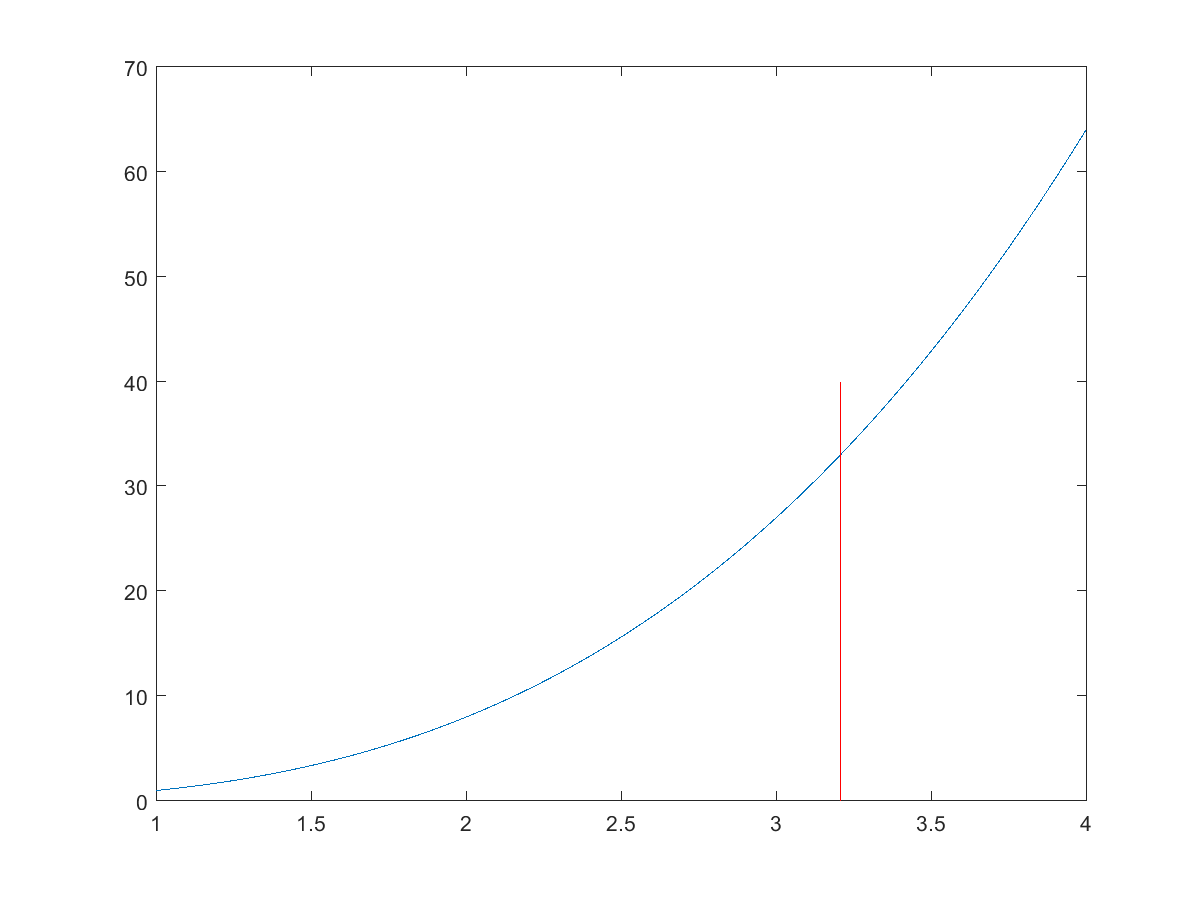
\includegraphics[width=0.4\linewidth]{graphics/Week06_IntegrationApplications/W06CenterOfMass1}
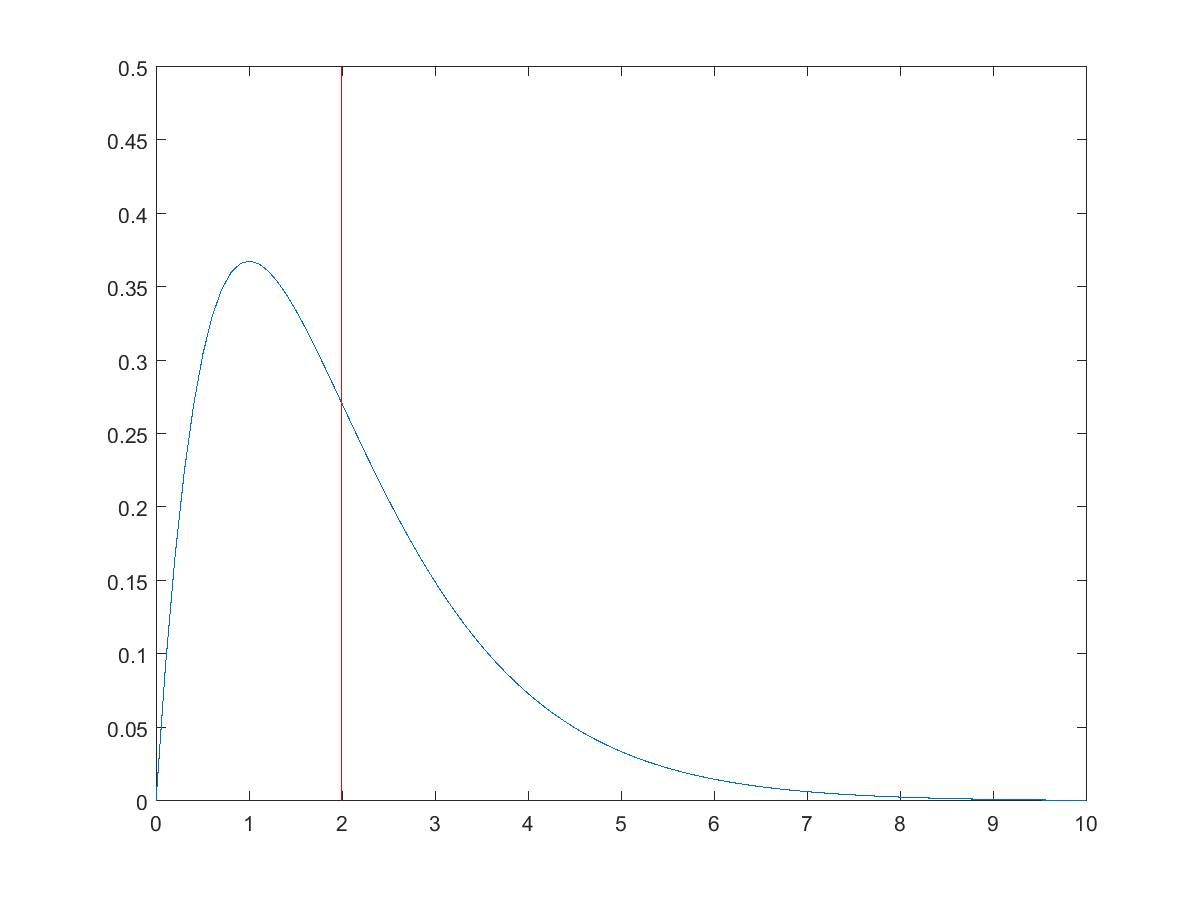
\includegraphics[width=0.4\linewidth]{graphics/Week06_IntegrationApplications/W06CenterOfMass2}
\end{center}

\end{Solution}

% ******************************
\item 
  \begin{Question}
    The width (in feet) of the golf course fairway was measured at
    100-foot intervals as indicated on the figure.  Estimate the
    square footage of of the fairway, using any appropriate means
    taught in the course.
    
    \begin{center}
      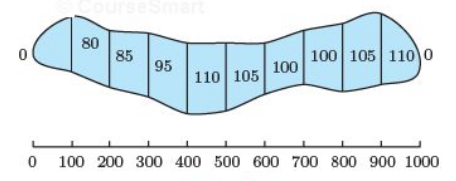
\includegraphics[width=0.5\linewidth]{graphics/Week06_IntegrationApplications/GolfHole}
    \end{center}
  \end{Question}
  
  
\begin{Solution}
  {\bf NOTE: } In this problem, because we are only given data and not
  a function, the only technique we have that would work is LEFT($n$).
  We {\bf can't} use the Fundamental Theorem or the \verb@integral@
  function because both of those require a formula for the function
  that we don't have.

The key steps are:
\begin{enumerate}[1.]
\item Create a vector of the widths, {\em including} the zero widths
  at the start and end of the fairway.
\item Note that  $\Delta x$ = 100 feet for each left-to-right distance.
\item Note that there are 10 intervals (11 widths), so we will be performing a LEFT(10) calculation.
\item Approximate the area on each left-to-right interval as
  $\mbox{width at the left} \times \Delta x$ (this is the LEFT rule on
  each interval).
\item Use a loop to accumulate the total area estimated.
\end{enumerate}

Link to the MATLAB code: \\
\href{http://www.mast.queensu.ca/~apsc171/MNTCP01/PracticeProblems/MATLAB/W06Golf.m}{W06Golf.m}

The final estimated area is 88,000 square feet.  We don't have a
formula for the widths, so this is simply our best estimate of the
area.

\end{Solution}


\hrulefill

\subsection*{Average Value}

\begin{multicols}{2}
%*****************
\item
  \begin{Question}
    \begin{enumerate}[(a)]
    \item Using the graph shown below, find $\ds \int^6_1 f(x)~dx$. 

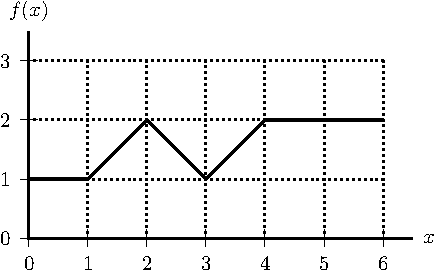
\includegraphics[width=0.9\linewidth]{graphics/Week06_AverageValue/average_1}
    \item What is the average value of $f$ on [1, 6]?
    \end{enumerate}
  \end{Question}

  \begin{Solution}
    The integral represents the area below the graph of $f(x)$ but above the $x$-axis.
    \begin{enumerate}[(a)]
    \item Since each square has area 1, by counting squares and half-squares we find
      \begin{align*}
\int^6_1 f(x) ~dx = 8.5.
      \end{align*}
(b) The average value is  \begin{align*}
\frac{1}{6 - 1} \int^6_1 f(x) ~dx 
& = \frac{8.5}{ 5 } = 1.7
\end{align*}
    \end{enumerate}
  \end{Solution}

%*****************
\item
  \begin{Question}
    \begin{enumerate}[(a)]
    \item Using the graph below, estimate $\ds \int^3_{-3} f(x) ~dx$. 
    \item  Which of the following average values of $f(x)$ is larger?  \\
      (i) Between $x = -3$ and $x = 3$, or   \\
      (ii) Between $x = 0$ and $x = 3$?
    \end{enumerate}
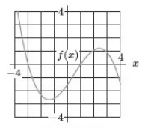
\includegraphics[width=0.7\linewidth]{graphics/Week06_AverageValue/average_2}
  \end{Question}

  \begin{Solution}
    \begin{enumerate}[(a)]
    \item The integral is the area above the $x$-axis minus the area
      below the $x$-axis. Thus, we can see that
      $\ds \int^3_{-3}f(x)~dx$ is about $-6 + 2 = -4$, based on \\
      the negative of the area from $t = -3$ to $t = 1$ plus the area
      from $t = 1$ to $t = 3$.  \\Note that your estimate may differ
      from this, depending on how you counted squares under the curved
      shape.
    \item Since the integral in part (a) is negative, the average
      value of $f(x)$ between $x = -3$ and $x = 3$ is negative. From
      the graph, however, it appears that the integral of $f(x)$ from
      $x = 0$ to $x = 3$ is positive overall, meaning that the average
      value will also be positive. Hence (ii) is the larger quantity.
    \end{enumerate}
  \end{Solution}
%*****************
\item
  \begin{Question}
    \begin{enumerate}[(a)]
    \item Using the graphs of $f(x)$ and $g(x)$ shown below, find the
      average value on $0 \le x \le 2$ of \\
      (i) $f(x)$ \hfill (ii) $g(x)$ \hfill (iii) $f( x) \cdot g(x)$ \\ \noindent
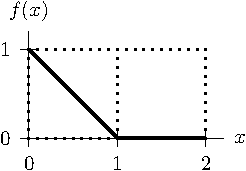
\includegraphics[width=0.5\linewidth]{graphics/Week06_AverageValue/average_product_graphs1}
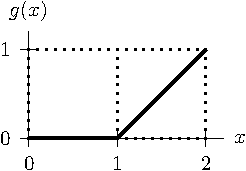
\includegraphics[width=0.5\linewidth]{graphics/Week06_AverageValue/average_product_graphs2}

    \item Is the statement that \begin{center}``Average($f$) $\cdot$ Average($g$) = Average($f \cdot g$)'' \end{center}true or not?  Explain your answer.
    \end{enumerate}
  \end{Question}

  \begin{Solution}
 (i) Since the triangular region under the graph of $f(x)$ has area $\ds \frac{1}{2}$, we have
 \begin{align*}
\mbox{Average}(f) &= \frac{1}{ 2 - 0} \int^2_0 f(x) ~dx 
& = \frac{1}{2} \cdot \frac{1}{2}
& = \frac{1}{4}
 \end{align*}
(ii) Similarly,
 \begin{align*}
\mbox{Average}(g) &= \frac{1}{2 - 0} \int^2_0 g(x) ~dx 
& = \frac{1}{2} \cdot \frac{1}{2}
& = \frac{1}{4}
 \end{align*}

 (iii) Since $f(x)$ is nonzero only for $0 \le x < 1$ and $g(x)$ is
 nonzero only for $1 < x \le 2$, the product $f(x)g(x)$ = 0 for all
 $x$. (To confirm this, try picking any $x$ value between 0 and 2, and
 subbing it into the expression $f(x) \cdot g(x)$.  

 Thus
\begin{align*}
\mbox{Average}(f \cdot g) & = \frac{1}{2 - 0} \int^2_0 f(x)g(x) ~dx 
& = \frac{1}{2} \int^2_0 0 ~dx = 0.
\end{align*}
(b) Since the average values of $f(x)$ and $g(x)$ are nonzero, their
product is nonzero. Thus the left side of the statement, Avg($f$)$\cdot$Avg($g$), is
nonzero. However, the average of the product $f(x)g(x)$ is zero. Thus,
the right side of the statement is zero, so the statement is not true.
  \end{Solution}
%*****************
\item
  \begin{Question}
    \begin{enumerate}[(a)]
    \item Without computing any integrals, explain why the average
      value of $f(x) = \sin x$ on $[0, \pi]$ must be between 0.5 and 1.
    \item Compute the exact average of $\sin x$ on $[0, \pi]$.
    \item Use MATLAB to plot the graph of $\sin(x)$ on $[0, \pi]$, and
      draw the average value on the graph as well.
    \end{enumerate}
  \end{Question}

  \begin{Solution}
    \begin{enumerate}[(a)]
    \item Since $f(x) = \sin x$ over $[0, \pi]$ is between 0 and 1,
      the average of $f(x)$ must itself be between 0 and
      1. Furthermore, since the graph of $f(x)$ is concave down on
      this interval, the average value must be greater than the
      average height of the triangle shown in the figure below, namely
      $y = 0.5$.

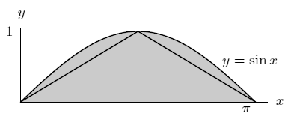
\includegraphics[width=0.7\linewidth]{graphics/Week06_AverageValue/sin_average_solution}

\item Average =$\ds \frac{1 }{\pi-0}\int^\pi_0 \sin x ~dx \approx 0.64$.

\item \lstinputlisting[showstringspaces=false]{MATLAB/W06SineAverage.m}

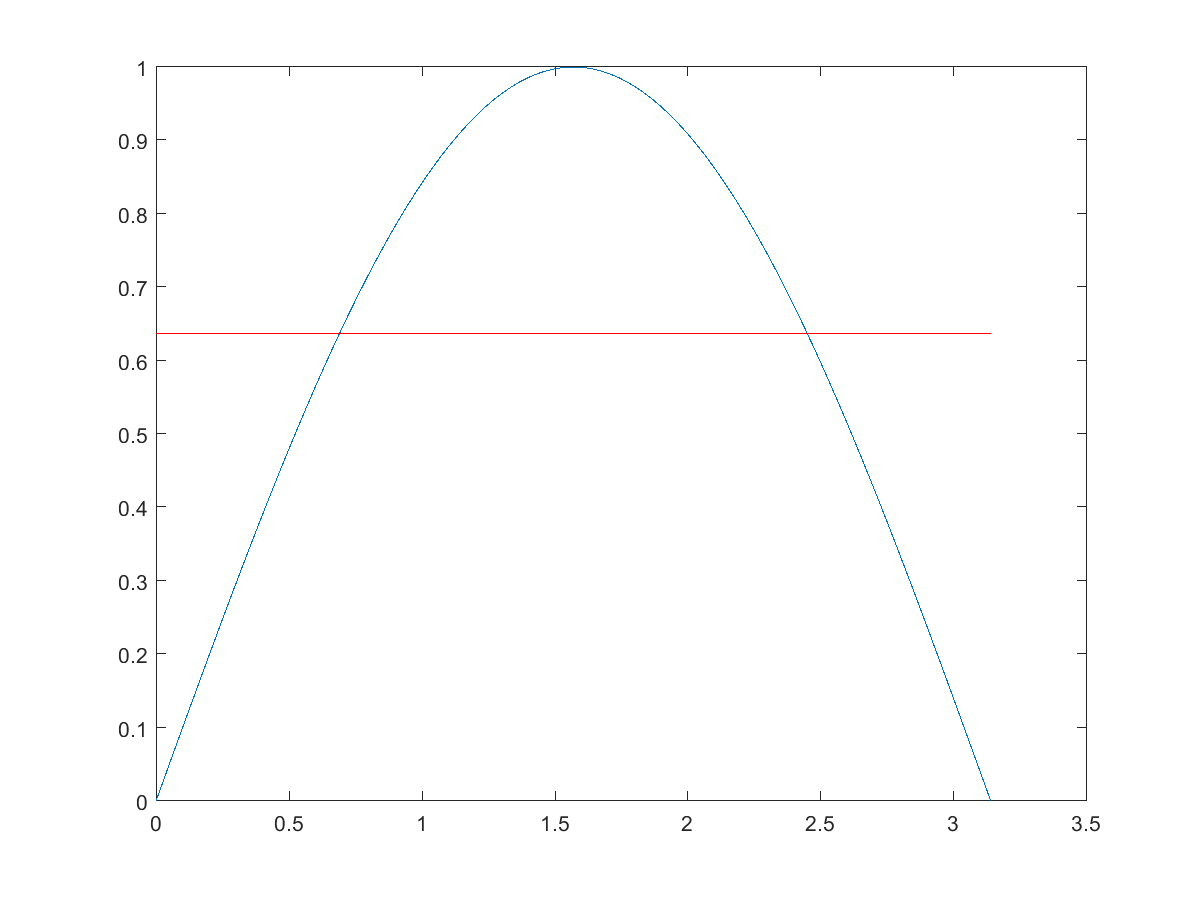
\includegraphics[width=0.9\linewidth]{graphics/Week06_AverageValue/W06SineAverage}
    \end{enumerate}
  \end{Solution}
%*****************
\item
  \begin{Question}
    \begin{enumerate}[(a)]
    \item What is the average value of $f(x) = \sqrt{ 1 - x^2}$ over
      the interval $0 \le x \le 1$?  (Hint: we don't have the
      integration tools to evaluate the integral of $f(x)$ from first
      principles, but can use MATLAB to evaluate it.)  
    \item Use MATLAB to plot the graph of $f(x)$ on $[0, 1]$, and draw
      the average value on the graph as well.
    \item How can you tell whether this average value is more or less
      than 0.5 without doing any calculations?
    \end{enumerate}
  \end{Question}

  \begin{Solution}
    \begin{enumerate}[(a)]
    \item Solution is computed in the script below, with the average value being 0.7854.

\item Graphing is also included in the script below. 

\href{http://www.mast.queensu.ca/~apsc171/MNTCP01/PracticeProblems/MATLAB/W06RootAverage.m}{W06RootAverage.m}

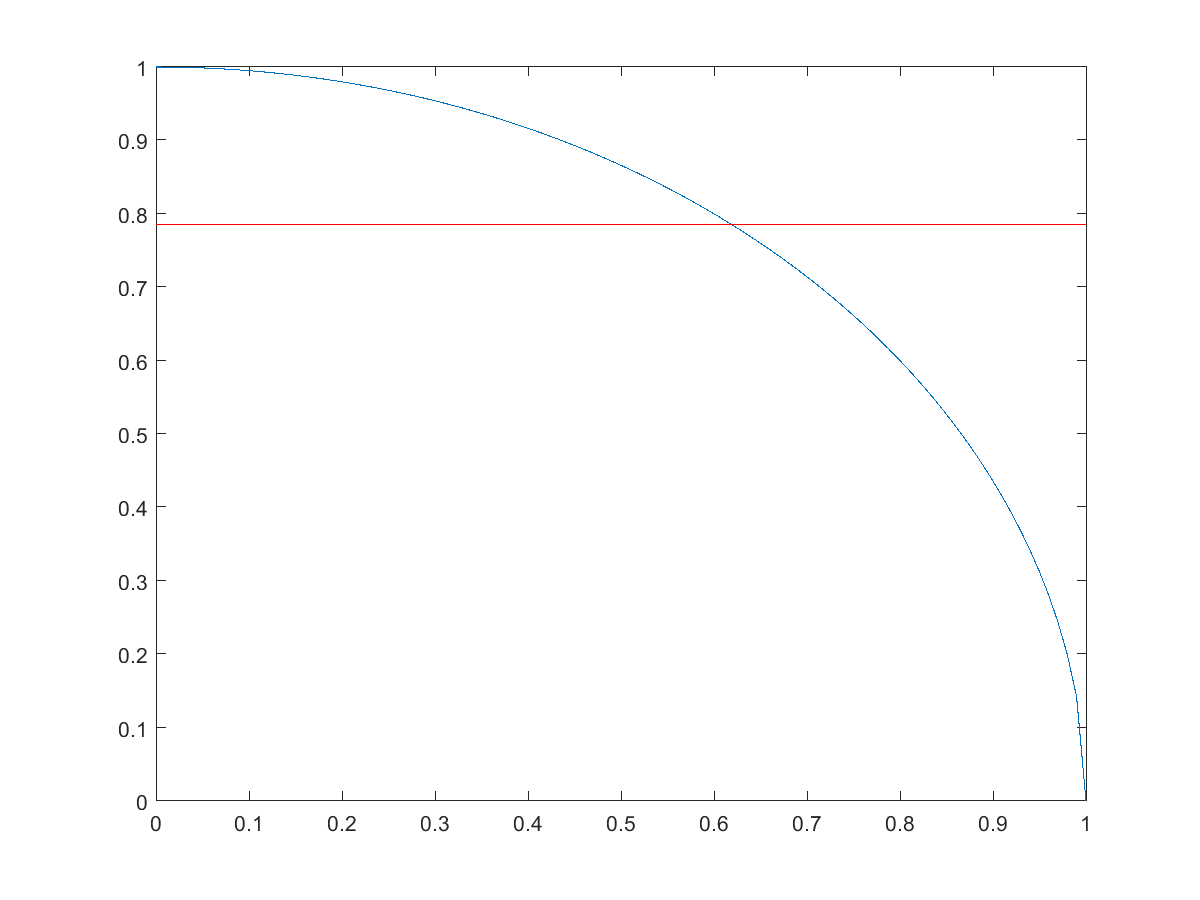
\includegraphics[width=0.7\linewidth]{graphics/Week06_AverageValue/W06RootAverage}

\item The area between the graph of $y = 1-x$ and the $x$-axis is
  0.5. Because the graph of $y = \sqrt{1 - x^2}$ is concave down, it
  lies above the straight line $y = 1 - x$, so its average value is
  above 0.5. See the figure below.

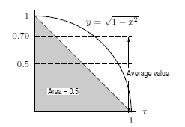
\includegraphics[width=0.7\linewidth]{graphics/Week06_AverageValue/circle_average_solution}
    \end{enumerate}
  \end{Solution}
\end{multicols}


\end{enumerate}
\end{document}

